% !TeX spellcheck = en_US
\section{Partial Pairwise Comparison Table}\label{section:pct}

In this section we will describe generated .isf and .apx file for Partial Pairwise Comparison Table. You can open this files by double clicking on them in workspace tree.

\subsection{Isf file}\label{sub:pct-isf}

This isf file is read only. Each row represents comparison of pair of examples. Each column represents attribute (criteria) on with comparison was performed.

\begin{figure*}[!ht] 
	\centering
	\makebox[\textwidth]{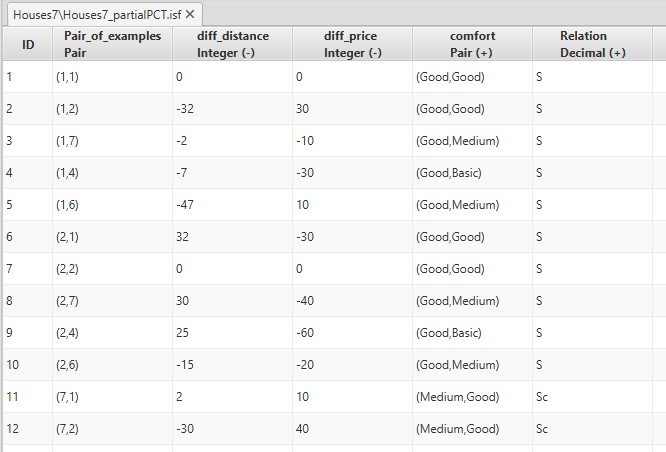
\includegraphics[width=.6\paperwidth]{raw/pct-isf}}
	\caption{Read only Partial Pairwise Comparison Table from Houses7}
\end{figure*}

In table header, field types and cost/gain criterion indicator is displayed. If you hover over column header, more information can be displayed. Columns can be ordered and sorted, but it will not be saved to file, because it is read only. You can also export selected rows to CSV format. You can do this by selecting rows and choosing ''Copy selected rows'' option from context menu.

\subsection{Apx file}\label{sub:pct-apx}

In this file additional information is saved in text format. User interface for this file is not created yet. It contains domination cons (P-dominating sets, P-dominated sets), approximations, decision classes and some metrics, like accuracy or quality of sorting.

\vfill\newpage